% Generated from tex/chapters/ch04/08_構築技術.tex for the SWEBOK structure tree
\subsubsection{性能分析とチューニング}

性能は、アーキテクチャ、詳細設計、データ構造、アルゴリズム、コードの書き方に影響される。性能分析は、プログラムの実行時情報を集め、時間がかかっている箇所、頻繁に実行される箇所、資源を多く使う箇所を見つける活動である。

コードチューニングは、コードレベルで性能を改善することである。論理式、ループ、データ変換、関数呼び出し、メモリアクセスなどを見直す。重要なのは、推測ではなく測定に基づいて行うことである。測定せずに最適化すると、本当に遅い場所ではない箇所を複雑にしてしまう危険がある。

\begin{keybox}{性能改善の原則}
まず測定し、ボトルネックを特定し、小さく変更し、再測定する。性能のために可読性を大きく下げる場合は、その理由と測定結果を残す必要がある。
\end{keybox}

\begin{figure}[htbp]
\centering
\IfFileExists{assets/generated_figures/ch04/fig-ch04-13.png}{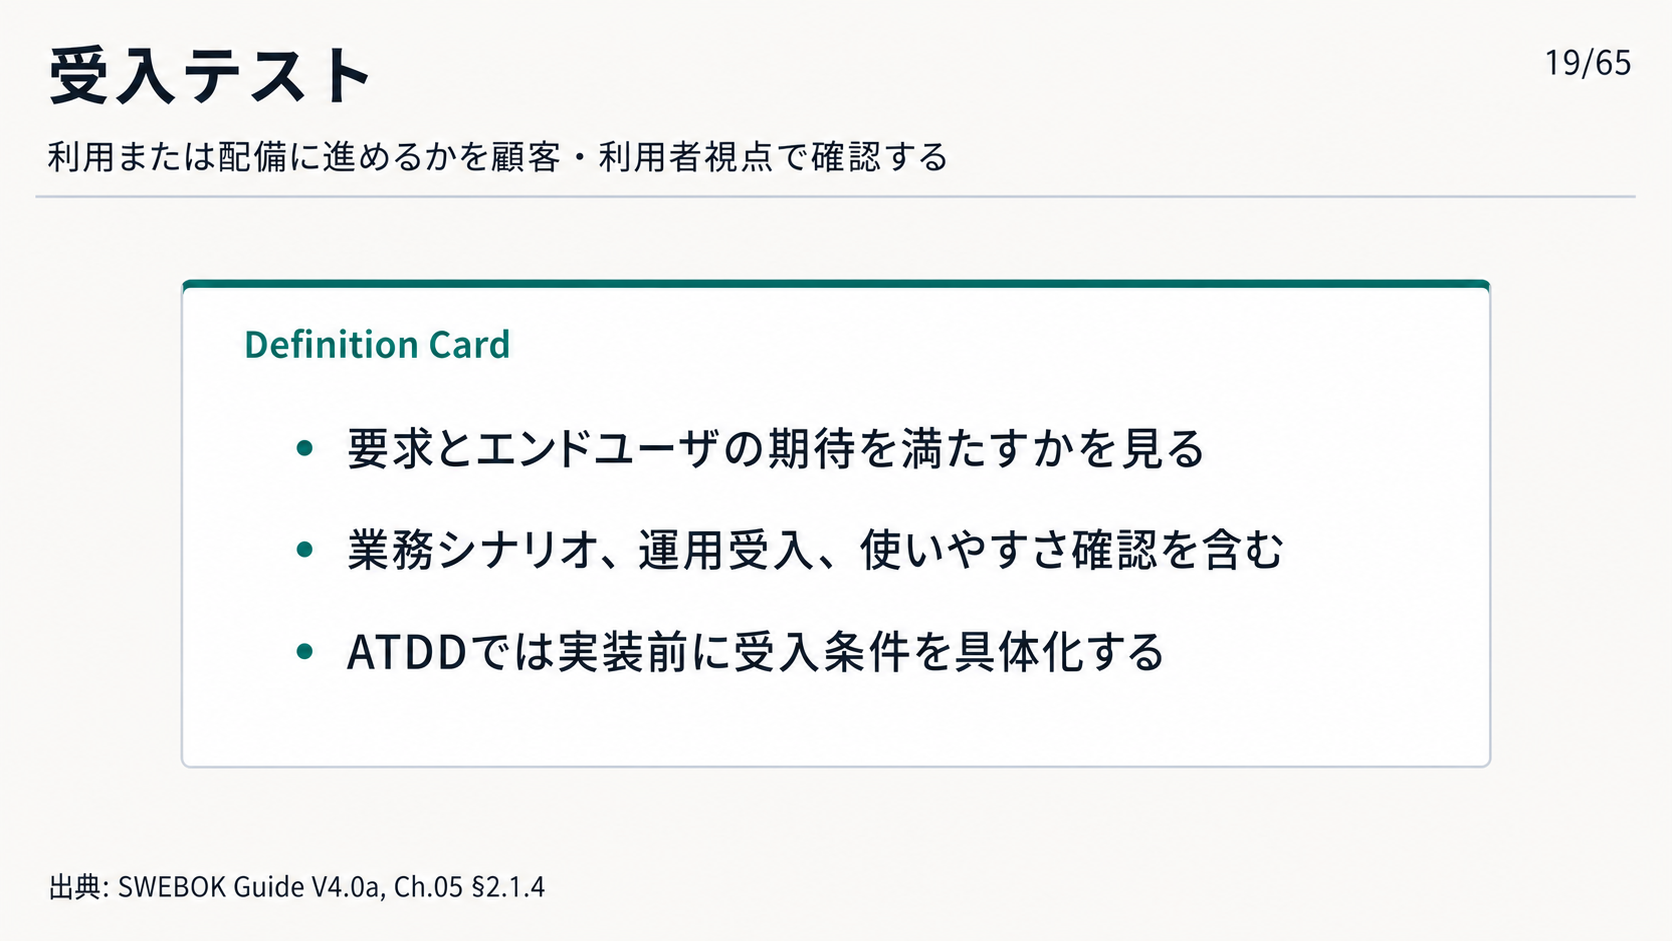
\includegraphics[width=0.96\linewidth]{assets/generated_figures/ch04/fig-ch04-13.png}}{\fbox{\parbox[c][48mm][c]{0.9\linewidth}{\centering 画像生成待ち\\性能分析とチューニングの流れ}}}
\caption{性能分析とチューニングの流れ}
\label{fig:ch04-13}
\end{figure}
